\documentclass[
  manuscript=poster,  %% article (default), rescience, data, software, proceedings, poster
  layout=preprint,  %% preprint (for submission) or publish (for publisher only)
  year=2026,
  volume=x,
]{extra/joas}

\doi{xx.xxxxx/joas.xxxx.xxxx}

% \conference{} command is only used for proceedings
\conference{The 14th OpenSky Symposium}

\received {1 April 20xx}
\revised  {1 May 20xx}
\accepted {10 May 20xx}
\published{20 May 20xx}

\editor{Editor Name}

\reviewers{First Reviewer, Second Reviewer, Third Reviewer}

% specify the .bib file for references
\addbibresource{reference.bib}
\usepackage{subfigure}
\usepackage{qrcode}
\usepackage{xurl}
\newcommand{\dataArchiveUrl}{https://doi.org/10.5281/zenodo.23090597}
\newcommand{\codeArchiveUrl}{https://doi.org/10.5281/zenodo.23089559}

% data values: every number in the text is a macro generated from numbers.json
% BEGIN GENERATED NUMBERS
% numbers.tex: GENERATED by scripts/gen_numbers_tex.py from numbers.json. DO NOT EDIT.
% Every data value in the paper and poster is read from these macros.
\newcommand{\aircraftGain}{9.3}
\newcommand{\aneelDec}{9.30}
\newcommand{\aneelFec}{4.66}
\newcommand{\aneelYear}{2025}
\newcommand{\antennaAltitude}{1,030}
\newcommand{\antennaHeightAgl}{4}
\newcommand{\azimuthBinDeg}{10}
\newcommand{\blindSectorEnd}{350}
\newcommand{\blindSectorShareEraA}{3.6}
\newcommand{\blindSectorShareEraB}{3.6}
\newcommand{\blindSectorStart}{290}
\newcommand{\brAircraftCount}{2,769}
\newcommand{\brAircraftShare}{56.2}
\newcommand{\brBlockEnd}{E7FFFF}
\newcommand{\brBlockStart}{E40000}
\newcommand{\brPositionCount}{30,938,487}
\newcommand{\brPositionShare}{84.7}
\newcommand{\commonFleetDeltaMean}{29.5}
\newcommand{\commonFleetDeltaMedian}{24.1}
\newcommand{\commonFleetDeltaPFive}{-36.6}
\newcommand{\commonFleetDeltaPNinetyFive}{114.6}
\newcommand{\commonFleetDeltaPositivePct}{81.6}
\newcommand{\commonFleetGain}{15.6}
\newcommand{\commonFleetMeanA}{188.5}
\newcommand{\commonFleetMeanB}{217.9}
\newcommand{\commonFleetMeanDefinition}{mean of all position ranges}
\newcommand{\commonFleetMilExcluded}{58}
\newcommand{\commonFleetN}{2,234}
\newcommand{\commonFleetPlotted}{2,176}
\newcommand{\commonFleetPlottedGain}{15.1}
\newcommand{\commonFleetPlottedMeanA}{195.4}
\newcommand{\commonFleetPlottedMeanB}{225.0}
\newcommand{\commonFleetPlottedMeanDefinition}{mean of per-aircraft mean ranges}
\newcommand{\commonFleetPlottedPooledGain}{15.3}
\newcommand{\commonFleetPlottedPooledMeanA}{191.4}
\newcommand{\commonFleetPlottedPooledMeanB}{220.7}
\newcommand{\dailyMaxDays}{138}
\newcommand{\dailyMaxEvents}{5}
\newcommand{\dailyMaxNonDuctDayMax}{581.4}
\newcommand{\ductClusterGapHours}{6}
\newcommand{\ductClusterStrictCount}{4}
\newcommand{\ductEventCount}{3}
\newcommand{\ductEventOneDates}{16 to 18 June}
\newcommand{\ductEventOnePoints}{1,060}
\newcommand{\ductEventOneWindowPoints}{1,062}
\newcommand{\ductEventThreeDate}{25 August}
\newcommand{\ductEventTwoDate}{15 August}
\newcommand{\ductPositionsTotal}{1,210}
\newcommand{\ductThresholdKm}{600}
\newcommand{\earthRadiusKm}{6371.0088}
\newcommand{\eraAAircraft}{2,890}
\newcommand{\eraADays}{32}
\newcommand{\eraAEnd}{2026-05-14}
\newcommand{\eraAMax}{510.3}
\newcommand{\eraAMedian}{189.3}
\newcommand{\eraAPNinetyFive}{299.7}
\newcommand{\eraAPositions}{5,153,167}
\newcommand{\eraAStart}{2026-04-13}
\newcommand{\eraBCalendarDates}{138}
\newcommand{\eraBEnd}{2026-09-30}
\newcommand{\eraBFirstPointUtc}{21:51}
\newcommand{\eraBFullAircraft}{4,925}
\newcommand{\eraBFullDays}{137}
\newcommand{\eraBFullMax}{786.3}
\newcommand{\eraBFullMaxNoDucting}{599.9}
\newcommand{\eraBFullMedian}{222.0}
\newcommand{\eraBFullPNinetyFive}{350.1}
\newcommand{\eraBFullPNinetyFiveRounded}{350}
\newcommand{\eraBFullPositions}{36,535,422}
\newcommand{\eraBHours}{3290.4}
\newcommand{\eraBLiveDays}{33}
\newcommand{\eraBLiveStart}{2026-08-29}
\newcommand{\eraBMaxDate}{17 June}
\newcommand{\eraBPairedAircraft}{3,159}
\newcommand{\eraBPairedDays}{32}
\newcommand{\eraBPairedEnd}{2026-06-17}
\newcommand{\eraBPairedMax}{786.3}
\newcommand{\eraBPairedMedian}{224.0}
\newcommand{\eraBPairedPNinetyFive}{350.6}
\newcommand{\eraBPairedPositions}{8,123,970}
\newcommand{\eraBStart}{2026-05-16}
\newcommand{\francaUrbanElevation}{1,040}
\newcommand{\gapBucketLongMin}{60}
\newcommand{\gapBucketShortMin}{15}
\newcommand{\gapCount}{40}
\newcommand{\gapDowntimeHours}{21.91}
\newcommand{\gapHourFiveCount}{6}
\newcommand{\gapHourSixCount}{13}
\newcommand{\gapMidCount}{5}
\newcommand{\gapNightData}{19}
\newcommand{\gapNightEndBrt}{04:00}
\newcommand{\gapNightEndUtc}{07:00}
\newcommand{\gapNightFrozen}{38}
\newcommand{\gapNightOverlapData}{20}
\newcommand{\gapNightStartBrt}{02:00}
\newcommand{\gapNightStartUtc}{05:00}
\newcommand{\gapOutageCount}{2}
\newcommand{\gapOverSixtyCount}{3}
\newcommand{\gapOverstateFactor}{20}
\newcommand{\gapShortCount}{32}
\newcommand{\gapThirdDate}{30 August}
\newcommand{\gapThirdMinutes}{64}
\newcommand{\gapThresholdS}{120}
\newcommand{\gapWindowHours}{3290.4}
\newcommand{\hexbinRingOneKm}{100}
\newcommand{\hexbinRingThreeKm}{500}
\newcommand{\hexbinRingTwoKm}{250}
\newcommand{\icmsHighPct}{20}
\newcommand{\icmsLowPct}{17}
\newcommand{\idecCenterWestDec}{15}
\newcommand{\idecCenterWestFec}{7}
\newcommand{\idecNorthDec}{24}
\newcommand{\idecNorthFec}{12}
\newcommand{\idecNortheastDec}{13}
\newcommand{\idecNortheastFec}{5}
\newcommand{\idecSouthDec}{10}
\newcommand{\idecSouthFec}{6}
\newcommand{\idecSoutheastDec}{7}
\newcommand{\idecSoutheastFec}{4}
\newcommand{\idecYear}{2022}
\newcommand{\importAltDeductionUsd}{0}
\newcommand{\importAltDutyPct}{60}
\newcommand{\importAltDutyUsd}{90}
\newcommand{\importAltIcmsUsd}{49}
\newcommand{\importAltMarkupPct}{93}
\newcommand{\importAltTotalUsd}{289}
\newcommand{\importAltTotalUsdExact}{289.16}
\newcommand{\importDeductionUsd}{30}
\newcommand{\importDutyPct}{60}
\newcommand{\importDutyUsd}{60}
\newcommand{\importExemptUsd}{50}
\newcommand{\importIcmsPct}{17}
\newcommand{\importIcmsUsd}{43}
\newcommand{\importKitUsd}{150}
\newcommand{\importMarkupPct}{69}
\newcommand{\importMaxUsd}{3,000}
\newcommand{\importTotalUsd}{253}
\newcommand{\importTotalUsdExact}{253.01}
\newcommand{\osnRefRangeHigh}{500}
\newcommand{\osnRefRangeLow}{400}
\newcommand{\outageAnnualHours}{40}
\newcommand{\outageAugDate}{2 August}
\newcommand{\outageAugHours}{9}
\newcommand{\outageAugMinutes}{47}
\newcommand{\outageJulDate}{6 July}
\newcommand{\outageJulHours}{5}
\newcommand{\outageJulMinutes}{12}
\newcommand{\outageTotalHours}{15}
\newcommand{\outageTotalHoursExact}{14.98}
\newcommand{\peakSectorEnd}{200}
\newcommand{\peakSectorStart}{140}
\newcommand{\posGain}{57.7}
\newcommand{\posGainExact}{57.65}
\newcommand{\readsbVersion}{3.16.14}
\newcommand{\receiverDowntimeHours}{14.99}
\newcommand{\receiverUptimePct}{99.54}
\newcommand{\receptionGapOffNightCount}{19}
\newcommand{\receptionGapOtherCount}{38}
\newcommand{\receptionGapOtherHours}{6.92}
\newcommand{\receptionUptimePct}{99.33}
\newcommand{\recvLat}{-20.51}
\newcommand{\recvLon}{-47.40}
\newcommand{\recvRoundingErrorKm}{1}
\newcommand{\sdrModel}{AirNav ADS-B 1090 MHz FlightStick}
\newcommand{\sensorSerial}{-1408044782}
\newcommand{\surveyBrazil}{6}
\newcommand{\surveyCostReasons}{58}
\newcommand{\surveyCostShare}{15.5}
\newcommand{\surveyCountryIdentified}{561}
\newcommand{\surveyLatam}{11}
\newcommand{\surveyMalePct}{94}
\newcommand{\surveyNonOwnerReasons}{375}
\newcommand{\surveyPowerReasons}{34}
\newcommand{\surveyPowerShare}{9.1}
\newcommand{\surveyUniversityPct}{76}
\newcommand{\swapDate}{2026-05-16}
\newcommand{\swapTimeBrt}{18:35}
\newcommand{\swapTimeUtc}{21:35}
\newcommand{\uptimePct}{99.33}
% END GENERATED NUMBERS

% below is the area for authors

% Title within 12 words (current title has 15; kept to match the programme)
\title{Operating a Volunteer OpenSky Node in Brazil: Field Notes on Coverage, Uptime, and Local Regulations}

\author{Eliel Felipe Junior \orcid{0000-0002-6333-1187}}
\affiliation{Independent contributor, OpenSky Network community, Franca, Brazil}
\email{eliel@saberlegal.com.br}

% maximum five keywords
\keywords{ADS-B; crowdsourcing; receiver coverage; Brazil; regulation}

\begin{document}

\begin{abstract}
This field report documents a volunteer OpenSky receiver in Franca, Brazil, using local ADS-B traces through September 2026. Replacing a home-built antenna with an AirNav XBoost raised median range from \eraAMedian{} to \eraBFullMedian~km. In matched windows, pooled mean range increased by \commonFleetGain\% for \commonFleetN{} aircraft observed with both antennas. A persistent blind sector suggests local obstruction; \ductEventCount{} exceptional propagation windows exceeded \ductThresholdKm~km. Reception continuity was \receptionUptimePct\%, while uptime based on two identified receiver outages was \receiverUptimePct\%. The operator reports power, software and thermal interruption causes without event-level attribution. Regional electricity indicators and an illustrative import-cost calculation contextualise the installation. The findings describe one receiver, not Brazilian or network-wide coverage; archived aggregates and scripts accompany the poster.
\end{abstract}

\section{Motivation and installation}
The OpenSky Network relies on volunteers maintaining their own receivers. Its user survey identifies cost as a major barrier in under-represented regions \cite{inauen2026citizen}. This case study connects antenna performance, operational continuity and practical onboarding constraints at sensor $\sensorSerial$ in Franca.

Franca, in north-eastern S\~ao Paulo, southeastern Brazil, is among the state's higher-elevation cities, approximately \francaUrbanElevation~m above sea level, with urban hills separated by stream valleys \cite{franca2026relevo}. The antenna is at approximately $\recvLat^{\circ}$, $\recvLon^{\circ}$, \antennaAltitude~m above sea level and \antennaHeightAgl~m above ground. A Raspberry Pi~5 runs ultrafeeder (readsb \readsbVersion) with an \sdrModel{} SDR. A home-built antenna was replaced by an AirNav XBoost on \swapDate{} at \swapTimeUtc~UTC.

\section{Data and coverage}
Era~A covers \eraAStart{} to \eraAEnd{} (\eraADays{} days); Era~B covers the swap to \eraBEnd{} (approximately \eraBFullDays{} days, including a partial first day). Analysis uses local readsb traces, not OpenSky database records. Only \texttt{adsb\_icao} and \texttt{adsb\_icao\_nt} positions are retained; multilateration is excluded. Ranges use haversine distance ($R=\earthRadiusKm$~km) from the archived rounded origin $\recvLat$, $\recvLon$. Its approximately \recvRoundingErrorKm~km rounding error is retained for consistency with the archived results \cite{felipe2026repo}.

Table~\ref{tb:eras} separates the full record from equal-length comparisons. In Era~A and the paired Era~B window, the common fleet of \commonFleetN{} aircraft had pooled mean ranges of \commonFleetMeanA{} and \commonFleetMeanB~km (+\commonFleetGain\%). The paired window yielded \posGain\% more positions and \aircraftGain\% more aircraft. Matching aircraft and window length reduces fleet-composition differences, but does not eliminate changes in routes or traffic.

\begin{table}[htbp!]
\centering\small
\caption{ADS-B metrics. Paired Era~B spans \eraBPairedDays{} days after the swap. Both Era~B maxima include the \eraBMaxDate{} propagation event.}
\label{tb:eras}
\begin{tabular}{lrrr}
\toprule
\textbf{Metric} & \textbf{Era A} & \textbf{B paired} & \textbf{B full} \\
\midrule
Days & \eraADays & \eraBPairedDays & \eraBFullDays \\
Positions & \eraAPositions & \eraBPairedPositions & \eraBFullPositions \\
Aircraft & \eraAAircraft & \eraBPairedAircraft & \eraBFullAircraft \\
Median (km) & \eraAMedian & \eraBPairedMedian & \eraBFullMedian \\
P95 (km) & \eraAPNinetyFive & \eraBPairedPNinetyFive & \eraBFullPNinetyFive \\
Maximum (km) & \eraAMax & \eraBPairedMax & \eraBFullMax \\
\bottomrule
\end{tabular}
\end{table}

Figure~\ref{fig:coverage} shows a blind sector from \blindSectorStart\textdegree{} to \blindSectorEnd\textdegree{} with both antennas, consistent with terrain or local obstruction. Coverage peaks at \peakSectorStart\textdegree{} to \peakSectorEnd\textdegree{}, towards S\~ao Paulo. The \ductEventCount{} declared ducting windows with positions beyond \ductThresholdKm~km were \ductEventOneDates{}, \ductEventTwoDate{} and \ductEventThreeDate{}. Maximum observed range was \eraBFullMax~km; excluding the exceptional positions within these windows gives \eraBFullMaxNoDucting~km. These observations do not establish the long-term frequency of ducting.

\begin{figure}[htbp!]
\centering
\subfigure[Era~B density; rings at \hexbinRingOneKm, \hexbinRingTwoKm{} and \hexbinRingThreeKm~km]{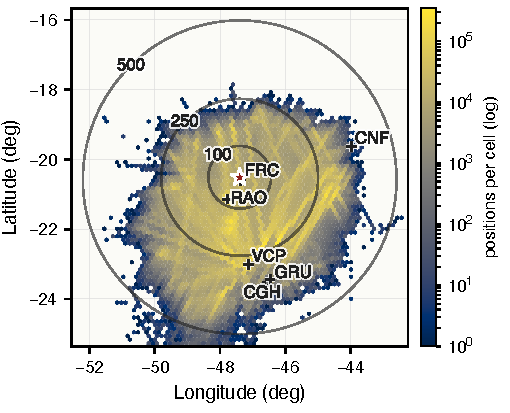
\includegraphics[width=0.46\textwidth]{figures/coverage_era_b_hexbin.pdf}}
\hfill
\subfigure[Position share (top) and P95 range (bottom), \azimuthBinDeg\textdegree{} azimuth bins]{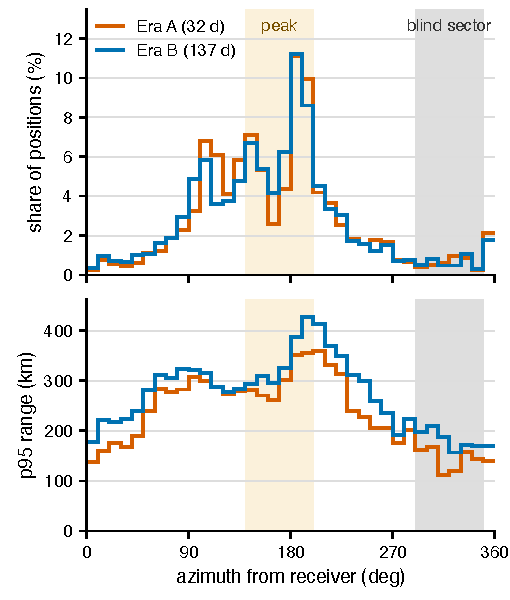
\includegraphics[width=0.46\textwidth]{figures/azimuth_range_ab.pdf}}
\caption{Local ADS-B coverage in Franca. Receiver origin rounded to two decimals. Traffic density is not guaranteed reception coverage.}
\label{fig:coverage}
\end{figure}

\section{Continuity and operating constraints}
Across \eraBHours~h, \gapCount{} reception gaps above \gapThresholdS~s totalled \gapDowntimeHours~h, giving \receptionUptimePct\% reception continuity. Of these, \gapNightData{} began between \gapNightStartUtc{} and \gapNightEndUtc~UTC; available statistics cannot distinguish receiver failure from an absence of observable traffic. Two identified receiver outages lasted \outageJulHours~h \outageJulMinutes~min on \outageJulDate{} and \outageAugHours~h \outageAugMinutes~min on \outageAugDate{}. Counting only these gives \receiverUptimePct\% receiver uptime. A further \gapThirdMinutes-minute gap on \gapThirdDate{} remains unexplained.

The operator reports occasional power loss, k3s conflicts after updates and USB SDR-stick overheating beyond its operating limit. No event-by-event attribution or cause-specific downtime is available. Reception continuity must therefore be distinguished from receiver uptime and electricity reliability. Regional context also matters: average interruption duration per consumer in \idecYear{} was about \idecSoutheastDec~h in the Southeast and \idecNorthDec~h in the North \cite{idec2023energia}; one Southeast installation cannot represent Brazil.

Practical regulatory touchpoints include equipment homologation, home-location privacy and international data transfers; the companion checklist documents these issues \cite{felipe2026repo,lgpd2018}. ADS-B-only observations cover the equipped fleet; continental deployment and equipage policies are discussed by DECEA \cite{decea2024samig}. Import costs add a concrete barrier: the illustrative Remessa Conforme calculation for a US\$\importKitUsd{} kit adds US\$\importDutyUsd{} duty and approximately US\$\importIcmsUsd{} ICMS, grossed up at \importIcmsPct\%, for about US\$\importTotalUsd{} (+\importMarkupPct\%) \cite{mf2026portaria}. This is a scenario, not a quotation for every purchase.

\section{Conclusions and limitations}
The antenna change coincided with improved range and message capture, while persistent directional obstruction and mixed interruption causes remain operational constraints. Cost, information and regional electricity reliability merit separate investigation. This single-node record cannot rank national barriers or measure OpenSky coverage. The last \eraBLiveDays{} days lack a source checksum; export-file hashes do not resolve that provenance limitation. A prior audit with an apparent date-label error is not used.

\section*{Funding statement}
This work received no external funding.

\section*{Open data statement}
Raw receiver traces are openly archived as dataset v1.0.0 under CC BY 4.0, DOI \href{\dataArchiveUrl}{\nolinkurl{10.5281/zenodo.23090597}} \cite{felipe2026traces}. Aggregate metrics, figures, code and the regulatory checklist are archived as v5.0.0, DOI \href{\codeArchiveUrl}{\nolinkurl{10.5281/zenodo.23089559}} \cite{felipe2026repo}.

\section*{Reproducibility statement}
\noindent\begin{minipage}[t]{0.82\linewidth}
\vspace{0pt}
Restore the public trace archives into the documented directory structure and run the archived dataset-building and metric scripts to recompute results. Checksums verify the input files; scripts specify time windows and ADS-B filtering. The QR links to dataset v1.0.0.
\end{minipage}\hfill
\begin{minipage}[t]{0.15\linewidth}
\vspace{0pt}\centering
{\hypersetup{urlcolor=black}\color{black}\qrcode[height=16mm]{https://doi.org/10.5281/zenodo.23090597}}\\
{\scriptsize Open dataset}
\end{minipage}

\begingroup
\emergencystretch=2em
\printbibliography
\endgroup
\end{document}
